% ថ្នាក់ទី ១១ (វិទ្យាសាស្ត្រសង្គម) · ជំពូកទី ៥ · មេរៀនទី ២ · សៀវភៅ ទំព័រ ១៧៤–១៨៧
\chapter{អនុវត្តន៍នៃដេរីវេ}

\begin{objBox}[វត្ថុបំណង]
\begin{enumerate}[1]
  \item រកសមីការនៃបន្ទាត់ប៉ះនឹងក្រាបតាងអនុគមន៍នៅត្រង់ចំណុចមួយ
  \item សិក្សាទិសដៅអថេរភាពនៃអនុគមន៍ទៅតាមសញ្ញានៃដេរីវេ
  \item រកតម្លៃអតិបរមានិងអប្បបរមាធៀបនៃអនុគមន៍
  \item ដោះស្រាយចំណោទតម្លៃអតិបរមានិងអប្បបរមា
  \item រកចំណុចរបត់នៃក្រាបតាងអនុគមន៍ពហុធាដឺក្រេទី $3$
  \item រកល្បឿននៃចលនាដោយប្រើដេរីវេនៃអនុគមន៍ចម្ងាយចរ ។
\end{enumerate}
\end{objBox}

ក្នុងមេរៀននេះ គេនឹងសិក្សាពីការអនុវត្តនៃដេរីវេចំពោះការដោះស្រាយចំណោទបន្ទាត់ប៉ះនឹងក្រាបតាងអនុគមន៍ចំណុចមួយ ការសិក្សាទិសដៅអថេរភាពនៃអនុគមន៍ ការគណនាតម្លៃអតិបរមា តម្លៃអប្បបរមា ការរកចំណុចរបត់នៃខ្សែកោង និងការរកល្បឿននៃចលនាមួយ ។

\section{បន្ទាត់ប៉ះនឹងក្រាបតាងអនុគមន៍}

\begin{center}
\begin{tikzpicture}[scale=1.15]
  \draw[->] (-0.5,0) -- (6,0) node[right] {$x$};
  \draw[->] (0,-0.5) -- (0,5.5) node[above] {$y$};
  \draw[thick,red,domain=1.8:4.6,samples=40] plot (\x,{0.25*(\x-1.5)^2+1.6});
  \coordinate (M) at (3,{0.25*1.5^2+1.6});
  \draw[blue,thick] (0.6,{0.75*(0.6-3)+0.25*1.5^2+1.6}) -- (5.3,{0.75*(5.3-3)+0.25*1.5^2+1.6}) node[right] {$T$};
  \foreach \t/\n in {4.4/N,4/N_1,3.6/N_2} {
    \draw[blue!60] (M) -- ($(M)!1.35!(\t,{0.25*(\t-1.5)^2+1.6})$);
    \fill (\t,{0.25*(\t-1.5)^2+1.6}) circle (2pt) node[left] {\small $\n$};
  }
  \fill (M) circle (2.5pt) node[below right] {$M$};
  \draw[dotted] (3,0) node[below] {$x_0$} -- (M) -- (0,{0.25*1.5^2+1.6}) node[left] {$y_0$};
  \node[red] at (4.8,5.2) {$y = f(x)$};
\end{tikzpicture}
\end{center}

គេមានចំណុច $M(x_0, f(x_0))$ និង $N(x, f(x))$ នៅលើក្រាបតាងអនុគមន៍ $f$ ។ ខ្នាត់ $MN$ មានមេគុណប្រាប់ទិស $\dfrac{f(x) - f(x_0)}{x - x_0}$ ។ បើចំណុច $N$ ផ្លាស់ទីលើក្រាប ហើយខិតជិត $M$ នោះខ្នាត់ $MN$ ងាកទៅរកទីតាំងលីមីត $(MT)$ ដែលហៅថាបន្ទាត់ប៉ះនឹងក្រាបតាងអនុគមន៍ $f$ ត្រង់ចំណុច $M(x_0, f(x_0))$ ។

ក្នុងករណីនេះ មេគុណប្រាប់ទិសនៃបន្ទាត់ប៉ះ $(MT)$ គឺជាលីមីតនៃមេគុណប្រាប់ទិសរបស់ខ្នាត់ $MN$ កាលណា $x$ ខិតជិត $x_0$ គឺ
\[
\begin{gathered}
m = \lim_{x \to x_0}\frac{f(x) - f(x_0)}{x - x_0} \quad \text{ឬ}\\
m = f'(x_0) \text{ ។}
\end{gathered}
\]

\begin{formulaBox}[ជាទូទៅ]
មេគុណប្រាប់ទិសនៃបន្ទាត់ប៉ះនឹងក្រាបតាងអនុគមន៍ $f$ នៅត្រង់ $x_0$ ជាដេរីវេ $f$ នៅត្រង់ $x_0$ គឺ $m = f'(x_0)$ ។
\end{formulaBox}

ដោយបន្ទាត់ប៉ះ $MT$ កាត់តាមចំណុច $M(x_0, y_0)$ និងមានមេគុណប្រាប់ទិស $f'(x_0)$ នោះបន្ទាត់ប៉ះ $MT$ មានសមីការ
\[
\begin{gathered}
y - y_0 = f'(x_0)(x - x_0) \quad \text{ឬ}\\
y = f'(x_0)(x - x_0) + y_0 \text{ ។}
\end{gathered}
\]

\begin{example}[លំហាត់គំរូ]
អនុគមន៍ $f(x) = x^3 - x^2 + 2$ មានក្រាប $C$ ។
\begin{enumerate}[a]
  \item រកសមីការបន្ទាត់ប៉ះនឹងក្រាប $C$ ត្រង់ចំណុច $A(1, 2)$ ។
  \item បន្ទាត់ $L$ មានមេគុណប្រាប់ទិសស្មើ $5$ ហើយប៉ះនឹងក្រាប $C$ ។ រកកូអរដោនេនៃចំណុចប៉ះរវាង $L$ និង $C$ ហើយរកសមីការបន្ទាត់ប៉ះត្រង់នោះ ។
\end{enumerate}
\end{example}
\ans
\begin{enumerate}[a]
  \item គេមាន $x_0 = 1$, $y_0 = 2$ ។ $f'(x) = 3x^2 - 2x$ នោះ $f'(x_0) = f'(1) = 3\times 1^2 - 2\times 1 = 1$ ។ បន្ទាត់ប៉ះនឹងក្រាប $C$ ត្រង់ $A(1, 2)$ មានសមីការ $y - y_0 = f'(x_0)(x - x_0)$ ឬ $y - 2 = 1(x - 1)$ ។ ដូច្នេះ $y = x + 1$ ។
  \item តាង $(a, b)$ ជាកូអរដោនេនៃចំណុចប៉ះ ។ បន្ទាត់ប៉ះ $L$ មានមេគុណប្រាប់ទិស $f'(a) = 5$ និង $f'(a) = 3a^2 - 2a$ ។ គេបាន $3a^2 - 2a = 5$ ឬ $3a^2 - 2a - 5 = 0$ មានឫស $a_1 = -1$, $a_2 = \dfrac{5}{3}$ ។

  ចំពោះ $a = -1$ នោះ $b = (-1)^3 - (-1)^2 + 2 = 0$ ។ ចំពោះ $a = \dfrac{5}{3}$ នោះ $b = \left(\dfrac{5}{3}\right)^3 - \left(\dfrac{5}{3}\right)^2 + 2 = \dfrac{104}{27}$ ។ ដូច្នេះមានចំណុចប៉ះពីរ $(-1, 0)$ និង $\left(\dfrac{5}{3}, \dfrac{104}{27}\right)$ ។

  បន្ទាត់ប៉ះត្រង់ចំណុច $(-1, 0)$ មានសមីការ $L_1 : y - 0 = 5(x - (-1))$ ឬ $y = 5x + 5$ ។

  បន្ទាត់ប៉ះត្រង់ចំណុច $\left(\dfrac{5}{3}, \dfrac{104}{27}\right)$ មានសមីការ $L_2 : y - \dfrac{104}{27} = 5\left(x - \dfrac{5}{3}\right)$ ឬ $y = 5x - \dfrac{121}{27}$ ។
\end{enumerate}

\begin{pro}
\begin{enumerate}[a]
  \item រកសមីការបន្ទាត់ប៉ះនឹងក្រាបតាង $y = -x^2 + x + 3$ ត្រង់ $x = 2$ ។
  \item រកសមីការបន្ទាត់ប៉ះនឹងក្រាបតាង $y = -x^3 + 3x + 4$ ហើយស្របនឹងបន្ទាត់មានសមីការ $y = 3x$ ។
  \item រកសមីការបន្ទាត់ $D$ ដែលប៉ះនឹងក្រាប $C : y = x^3 - 4x$ ត្រង់ចំណុច $A(1, -3)$ ។ ទាញរកកូអរដោនេនៃចំណុចប្រសព្វមួយទៀតរវាងបន្ទាត់ $D$ និងក្រាប $C$ ។
\end{enumerate}
\ans
ក. $y = -3x + 7$ \quad ខ. $y = 3x + 4$ \quad គ. $D : y = -x - 2$ និងចំណុចប្រសព្វគឺ $(1, -3)$, $(-2, 0)$ ។
\end{pro}

\section{ទិសដៅអថេរភាពនៃអនុគមន៍}

ក្នុងផ្នែកនេះ យើងនឹងលើកយកមកសិក្សាពីវិធីងាយៗ សម្រាប់បញ្ជាក់ថាអនុគមន៍មួយកើន ឬចុះនៅក្នុងចន្លោះណាខ្លះ ។

\subsection{អនុគមន៍កើន-អនុគមន៍ចុះ}

\begin{center}
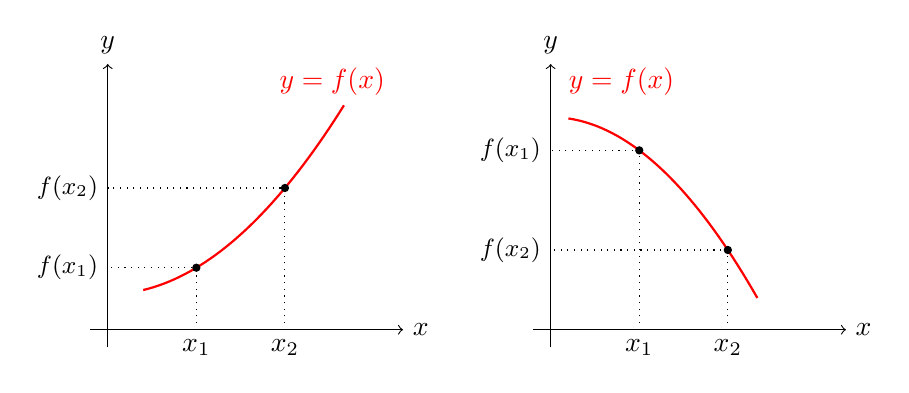
\begin{tikzpicture}[scale=0.75]
  \begin{scope}
  \draw[->] (-0.3,0) -- (5,0) node[right] {$x$};
  \draw[->] (0,-0.3) -- (0,4.5) node[above] {$y$};
  \draw[thick,red,domain=0.6:4,samples=40] plot (\x,{0.2*\x*\x+0.6});
  \fill (1.5,{0.2*2.25+0.6}) circle (2pt); \fill (3,{0.2*9+0.6}) circle (2pt);
  \draw[dotted] (1.5,0) node[below] {$x_1$} -- (1.5,1.05) -- (0,1.05) node[left] {\small $f(x_1)$};
  \draw[dotted] (3,0) node[below] {$x_2$} -- (3,2.4) -- (0,2.4) node[left] {\small $f(x_2)$};
  \node[red] at (3.8,4.2) {$y = f(x)$};
  \end{scope}
  \begin{scope}[xshift=7.5cm]
  \draw[->] (-0.3,0) -- (5,0) node[right] {$x$};
  \draw[->] (0,-0.3) -- (0,4.5) node[above] {$y$};
  \draw[thick,red,domain=0.3:3.5,samples=40] plot (\x,{3.6-0.25*\x*\x});
  \fill (1.5,{3.6-0.25*2.25}) circle (2pt); \fill (3,{3.6-0.25*9}) circle (2pt);
  \draw[dotted] (1.5,0) node[below] {$x_1$} -- (1.5,3.04) -- (0,3.04) node[left] {\small $f(x_1)$};
  \draw[dotted] (3,0) node[below] {$x_2$} -- (3,1.35) -- (0,1.35) node[left] {\small $f(x_2)$};
  \node[red] at (1.2,4.2) {$y = f(x)$};
  \end{scope}
\end{tikzpicture}
\end{center}

\begin{itemize}
  \item $f$ ជាអនុគមន៍កើននៅលើចន្លោះ $I$ មួយ កាលណា $\forall x_1, x_2 \in I$, $x_1 < x_2$ នាំឱ្យ $f(x_1) < f(x_2)$ ។
  \item $f$ ជាអនុគមន៍ចុះនៅលើចន្លោះ $I$ មួយ កាលណា $\forall x_1, x_2 \in I$, $x_1 < x_2$ នាំឱ្យ $f(x_1) > f(x_2)$ ។
\end{itemize}

\begin{example}[លំហាត់គំរូ]
បង្ហាញថាអនុគមន៍ $f(x) = x^2$ កើនចំពោះ $x > 0$ ហើយចុះចំពោះ $x < 0$ ។
\end{example}
\ans
ចំពោះ $0 < x_1 < x_2$ គេបាន $f(x_2) - f(x_1) = x_2^2 - x_1^2 = (x_2 + x_1)(x_2 - x_1) > 0$ ។ $f(x_2) - f(x_1) > 0$ នាំឱ្យ $f(x_1) < f(x_2)$ ។ ដូច្នេះ $f$ ជាអនុគមន៍កើនចំពោះ $x > 0$ ។

ចំពោះ $x_1 < x_2 < 0$ គេបាន $f(x_2) - f(x_1) = (x_2 + x_1)(x_2 - x_1) < 0$ ។ $f(x_2) - f(x_1) < 0$ នាំឱ្យ $f(x_1) > f(x_2)$ ។ ដូច្នេះ $f$ ជាអនុគមន៍ចុះចំពោះ $x < 0$ ។

\begin{pro}
\begin{enumerate}[a]
  \item បង្ហាញថា $y = x^3$ ជាអនុគមន៍កើនជានិច្ច ។
  \item តើអនុគមន៍ $y = 1 - x^2$ ជាអនុគមន៍កើនឬចុះ ចំពោះ $x > 0$ ។
\end{enumerate}
\ans
ក. ចំពោះ $x_1 < x_2$ ៖ $x_2^3 - x_1^3 = (x_2 - x_1)\left[\left(x_2 + \dfrac{x_1}{2}\right)^2 + \dfrac{3x_1^2}{4}\right] > 0$ \quad ខ. $y = 1 - x^2$ ជាអនុគមន៍ចុះ ចំពោះ $x > 0$ ។
\end{pro}

\subsection{ដេរីវេនិងទិសដៅអថេរភាពនៃអនុគមន៍}

បើគេពិនិត្យមើលក្រាប $(C_1)$ តាងអនុគមន៍ $f$ ដែលកើននៅលើចន្លោះ $(a, b)$ នោះគេសង្កេតឃើញថា បន្ទាត់ប៉ះទាំងអស់នឹងក្រាបមានមេគុណប្រាប់ទិសវិជ្ជមាន គឺមានន័យថា $f'(x) > 0$ ចំពោះគ្រប់ $x \in (a, b)$ ។ តាមរបៀបដូចគ្នាដែរ បន្ទាត់ប៉ះនឹងក្រាប $(C_2)$ តាងអនុគមន៍ចុះមានមេគុណប្រាប់ទិសអវិជ្ជមាន គឺបានន័យថា $f'(x) < 0$ ចំពោះគ្រប់ $x \in (a, b)$ ។

\begin{formulaBox}[ជាទូទៅ]
\begin{itemize}
  \item $f$ ជាអនុគមន៍កើននៅលើចន្លោះ $(a, b)$ លុះត្រាតែ $f'(x) > 0$ គ្រប់ $x \in (a, b)$ ។
  \item $f$ ជាអនុគមន៍ចុះនៅលើចន្លោះ $(a, b)$ លុះត្រាតែ $f'(x) < 0$ គ្រប់ $x \in (a, b)$ ។
  \item $f$ ជាអនុគមន៍ថេរនៅលើចន្លោះ $(a, b)$ លុះត្រាតែ $f'(x) = 0$ គ្រប់ $x \in (a, b)$ ។
\end{itemize}
\end{formulaBox}

\begin{example}[លំហាត់គំរូ ១]
កំណត់ចន្លោះដែលអនុគមន៍ $f(x) = 4x^3 + 5x - 9$ ជាអនុគមន៍កើន ។
\end{example}
\ans
ជំហានទី $1$ ៖ រកដេរីវេ $f'(x)$ គេបាន $f'(x) = 12x^2 + 5$ ។

ជំហានទី $2$ ៖ សិក្សាសញ្ញានៃ $f'(x)$ ។ ដោយ $12x^2 \ge 0$ ចំពោះគ្រប់ $x \in \mathbb{R}$ នោះ $f'(x) = 12x^2 + 5 > 0$ គ្រប់ $x \in \mathbb{R}$ ។ ដូច្នេះ $f$ ជាអនុគមន៍កើននៅលើ $\mathbb{R}$ ។

\begin{example}[លំហាត់គំរូ ២]
កំណត់តម្លៃ $m$ ដើម្បីឱ្យ $f(x) = (m - 1)x^2 + m^2 + m + 1$ ជាអនុគមន៍ចុះចំពោះ $x > 0$ ។
\end{example}
\ans
$f'(x) = 2(m - 1)x$ ។ ដើម្បីឱ្យ $f$ ជាអនុគមន៍ចុះ ចំពោះ $x > 0$ លុះត្រាតែ $f'(x) < 0$ ចំពោះ $x > 0$ $\Rightarrow 2(m - 1)x < 0$ តែ $x > 0$ $\Rightarrow m - 1 < 0$ នោះ $m < 1$ ។ ដូច្នេះ $m \in (-\infty, 1)$ ។

\begin{pro}
\begin{enumerate}[a]
  \item កំណត់ចន្លោះដែល $f(x) = -x^3 + x^2 + 5x - 6$ ជាអនុគមន៍កើនឬចុះ ។
  \item រកតម្លៃ $a$ ដើម្បីឱ្យ $g(x) = x^3 + ax^2 + \dfrac{1}{3}x - 4$ ជាអនុគមន៍កើនជានិច្ច ។
\end{enumerate}
\ans
ក. បើ $x \in (-\infty, -1) \cup \left(\dfrac{5}{3}, +\infty\right)$, $f$ ជាអនុគមន៍ចុះ ។ បើ $x \in \left(-1, \dfrac{5}{3}\right)$, $f$ ជាអនុគមន៍កើន ។ \quad ខ. $a \in (-1, 1)$ ។
\end{pro}

\section{អតិបរមាធៀបនិងអប្បបរមាធៀបនៃអនុគមន៍}
\subsection{អតិបរមាធៀប អប្បបរមាធៀប និងដេរីវេទី 1}

\begin{example}[ឧទាហរណ៍]
គេឱ្យអនុគមន៍ $f(x) = x^3 - 6x^2 + 9x - 2$ ។ គេបាន $f'(x) = 3x^2 - 12x + 9$ ។ បើ $f'(x) = 3x^2 - 12x + 9 = 0$ នោះ $x = 1$, $x = 3$ ។
\begin{center}
\begin{tikzpicture}
  \tkzTabInit[lgt=1.6,espcl=2]{$x$ /0.8, $f'(x)$ /0.8, $f(x)$ /1.6}{$-\infty$, $1$, $3$, $+\infty$}
  \tkzTabLine{, +, z, -, z, +, }
  \tkzTabVar{-/ , +/$2$, -/$-2$, +/ }
\end{tikzpicture}
\end{center}
តាមតារាងខាងលើ គេបាន $f(1) = 2$ ជាតម្លៃអតិបរមាធៀបនៃ $f$ ត្រង់ $x = 1$ ហើយ $f(3) = -2$ ជាតម្លៃអប្បបរមាធៀបនៃ $f$ ត្រង់ $x = 3$ ។
\end{example}

\begin{formulaBox}[ជាទូទៅ]
\begin{itemize}
  \item $f$ មានអតិបរមាធៀបត្រង់ $x_0$ កាលណា $f'(x) > 0$ ចំពោះ $x < x_0$, $f'(x_0) = 0$ និង $f'(x) < 0$ ចំពោះ $x > x_0$ ។ $f(x_0)$ ជាតម្លៃអតិបរមាធៀប ។
  \item $f$ មានអប្បបរមាធៀបត្រង់ $x_0$ កាលណា $f'(x) < 0$ ចំពោះ $x < x_0$, $f'(x_0) = 0$ និង $f'(x) > 0$ ចំពោះ $x > x_0$ ។ $f(x_0)$ ជាតម្លៃអប្បបរមាធៀប ។
\end{itemize}
\end{formulaBox}

\begin{center}
\begin{tikzpicture}[scale=0.7]
  \begin{scope}
  \draw[->] (-0.3,0) -- (4,0) node[right] {$x$}; \draw[->] (0,-0.3) -- (0,3.5) node[above] {$y$};
  \draw[thick,red,domain=1.5:3.5] plot (\x,{2.5-0.8*(\x-2.5)^2});
  \draw[dotted] (2.5,0) node[below] {$x_0$} -- (2.5,2.5) -- (0,2.5) node[left] {$f(x_0)$};
  \node at (2,-1) {\small $f(x_0)$ ជាតម្លៃអតិបរមាធៀប};
  \end{scope}
  \begin{scope}[xshift=7cm]
  \draw[->] (-0.3,0) -- (4,0) node[right] {$x$}; \draw[->] (0,-0.3) -- (0,3.5) node[above] {$y$};
  \draw[thick,red,domain=1.5:3.5] plot (\x,{1.2+0.8*(\x-2.5)^2});
  \draw[dotted] (2.5,0) node[below] {$x_0$} -- (2.5,1.2) -- (0,1.2) node[left] {$f(x_0)$};
  \node at (2,-1) {\small $f(x_0)$ ជាតម្លៃអប្បបរមាធៀប};
  \end{scope}
\end{tikzpicture}
\end{center}

\begin{example}[លំហាត់គំរូ ១]
បង្ហាញថាអនុគមន៍ $f(x) = -x^3 + 3x^2 + 1$ មានអតិបរមាធៀបនិងអប្បបរមាធៀប ហើយគណនាតម្លៃទាំងពីរនោះ ។
\end{example}
\ans
ជំហានទី $1$ ៖ រកដេរីវេ $f'(x) = -3x^2 + 6x$ ។

ជំហានទី $2$ ៖ សិក្សាសញ្ញានៃ $f'(x)$ ។ បើ $f'(x) = -3x^2 + 6x = 0$ ឬ $3x(-x + 2) = 0$ នោះ $x = 0$ ឬ $x = 2$ ។
\begin{center}
\begin{tikzpicture}
  \tkzTabInit[lgt=1.6,espcl=2]{$x$ /0.8, $f'(x)$ /0.8}{$-\infty$, $0$, $2$, $+\infty$}
  \tkzTabLine{, -, z, +, z, -, }
\end{tikzpicture}
\end{center}
ជំហានទី $3$ ៖ បកស្រាយពីការប្ដូរសញ្ញានៃ $f'(x)$ និងគណនាតម្លៃបរមា ។ តាមតារាងសញ្ញា $f'(x) = 0$ ត្រង់ $x = 0$ ហើយ $f'(x)$ ដូរសញ្ញាពី $-$ ទៅ $+$ ។ ដូច្នេះ $f$ មានអប្បបរមាធៀបត្រង់ $x = 0$ ហើយមានតម្លៃអប្បបរមាធៀបគឺ $f(0) = 1$ ។

ម្យ៉ាងទៀត $f'(x) = 0$ ត្រង់ $x = 2$ ហើយ $f'(x)$ ដូរសញ្ញាពី $+$ ទៅ $-$ ។ ដូច្នេះ $f$ មានអតិបរមាធៀបត្រង់ $x = 2$ ហើយតម្លៃអតិបរមាគឺ $f(2) = 5$ ។

\begin{example}[លំហាត់គំរូ ២]
រកតម្លៃ $m$ ដើម្បីឱ្យ $y = x^3 + 3mx^2 - mx + 1$ មានអតិបរមាធៀបនិងអប្បបរមាធៀប ។
\end{example}
\ans
ជំហានទី $1$ ៖ រកដេរីវេ $y' = 3x^2 + 6mx - m$ ។

ជំហានទី $2$ ៖ ដាក់លក្ខខណ្ឌដើម្បីឱ្យអនុគមន៍មានអតិបរមាធៀបនិងអប្បបរមាធៀប ។ អនុគមន៍មានអតិបរមាធៀបនិងអប្បបរមាធៀប លុះត្រាតែសមីការ $y' = 0$ មានឫសពីរផ្សេងគ្នាជាចំនួនពិត ។ សមីការ $3x^2 + 6mx - m = 0$ មានឫសពីរផ្សេងគ្នាជាចំនួនពិត លុះត្រាតែ $\Delta' = 9m^2 + 3m = 3m(3m + 1) > 0$ ។ បើ $3m(3m + 1) = 0$ នោះ $m = 0$ ឬ $m = -\dfrac{1}{3}$ ។
\begin{center}
\begin{tikzpicture}
  \tkzTabInit[lgt=1.6,espcl=2]{$m$ /0.8, $\Delta'$ /0.8}{$-\infty$, $-\frac{1}{3}$, $0$, $+\infty$}
  \tkzTabLine{, +, z, -, z, +, }
\end{tikzpicture}
\end{center}
ដូច្នេះ $m \in \left(-\infty, -\dfrac{1}{3}\right) \cup (0, +\infty)$ ។

\begin{pro}
រកតម្លៃ $k$ ដើម្បីឱ្យអនុគមន៍ $y = \dfrac{1}{3}x^3 + kx^2 + (2k + 3)x$ គ្មានបរមាធៀប ។
\ans
$k \in [-1, 3]$ ។
\end{pro}

\subsection{អតិបរមាធៀប អប្បបរមាធៀប និងដេរីវេទី 2}

\begin{center}
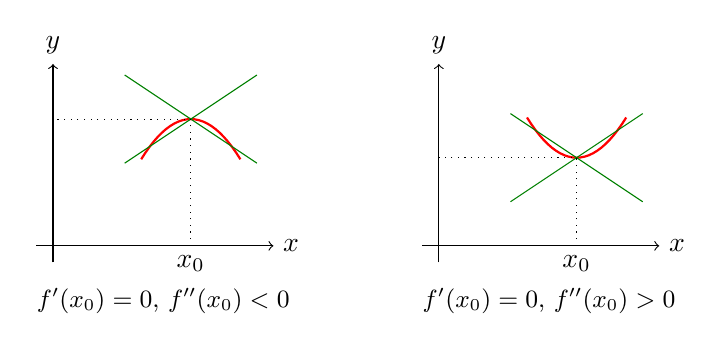
\begin{tikzpicture}[scale=0.7]
  \begin{scope}
  \draw[->] (-0.3,0) -- (4,0) node[right] {$x$}; \draw[->] (0,-0.3) -- (0,3.3) node[above] {$y$};
  \draw[thick,red,domain=1.6:3.4] plot (\x,{2.3-0.9*(\x-2.5)^2});
  \draw[green!50!black] (1.3,1.5) -- (3.7,3.1); \draw[green!50!black] (1.3,3.1) -- (3.7,1.5);
  \draw[dotted] (2.5,0) node[below] {$x_0$} -- (2.5,2.3) -- (0,2.3);
  \node at (2,-1) {\small $f'(x_0) = 0$, $f''(x_0) < 0$};
  \end{scope}
  \begin{scope}[xshift=7cm]
  \draw[->] (-0.3,0) -- (4,0) node[right] {$x$}; \draw[->] (0,-0.3) -- (0,3.3) node[above] {$y$};
  \draw[thick,red,domain=1.6:3.4] plot (\x,{1.6+0.9*(\x-2.5)^2});
  \draw[green!50!black] (1.3,0.8) -- (3.7,2.4); \draw[green!50!black] (1.3,2.4) -- (3.7,0.8);
  \draw[dotted] (2.5,0) node[below] {$x_0$} -- (2.5,1.6) -- (0,1.6);
  \node at (2,-1) {\small $f'(x_0) = 0$, $f''(x_0) > 0$};
  \end{scope}
\end{tikzpicture}
\end{center}

តាមក្រាបទី $1$ អនុគមន៍ $f$ មានអតិបរមាធៀបនៅត្រង់ចំណុចដែលក្រាបមានបន្ទាត់ប៉ះជាបន្ទាត់ដេក ហើយបន្ទាត់ប៉ះត្រង់ចំណុចផ្សេងទៀតនៃក្រាបដែលនៅជិតនោះ មានមេគុណប្រាប់ទិសថយចុះ គឺបានន័យថា $f'(x)$ ជាអនុគមន៍ចុះ ហើយ $f''(x) < 0$ ។

តាមក្រាបទី $2$ អនុគមន៍ $f$ មានអប្បបរមាធៀបនៅត្រង់ចំណុចដែលក្រាបមានបន្ទាត់ប៉ះជាបន្ទាត់ដេក ហើយបន្ទាត់ប៉ះត្រង់ចំណុចផ្សេងទៀតនៃក្រាបដែលនៅជិតនោះ មានមេគុណប្រាប់ទិសកើនឡើង គឺបានន័យថា $f'(x)$ ជាអនុគមន៍កើន ហើយ $f''(x) > 0$ ។

\begin{formulaBox}[ជាទូទៅ]
អនុគមន៍ $y = f(x)$ មានដេរីវេពីរដងលើចន្លោះមួយដែលមាន $x_0$ ។
\begin{itemize}
  \item $f$ មានអតិបរមាធៀបត្រង់ $x_0$ កាលណា $f'(x_0) = 0$ និង $f''(x_0) < 0$ ។
  \item $f$ មានអប្បបរមាធៀបត្រង់ $x_0$ កាលណា $f'(x_0) = 0$ និង $f''(x_0) > 0$ ។
\end{itemize}
\end{formulaBox}

\begin{note}[សម្គាល់]
បើ $f''(x_0) = 0$ នោះគេត្រូវត្រឡប់ទៅសិក្សាសញ្ញានៃដេរីវេទី $1$ វិញ ដើម្បីឈានទៅរកតម្លៃអតិបរមានិងអប្បបរមាធៀប ។
\end{note}

\begin{example}[លំហាត់គំរូ]
រកតម្លៃអតិបរមាធៀបនិងអប្បបរមាធៀបនៃ $f(x) = x^3 - 12x^2$ ។
\end{example}
\ans
ជំហានទី $1$ ៖ រកដេរីវេ $f'(x) = 3x^2 - 24x$ ។

ជំហានទី $2$ ៖ រកឫសនៃសមីការ $f'(x) = 3x^2 - 24x = 0$ ឬ $3x(x - 8) = 0$ នោះ $x = 0$ ឬ $x = 8$ ។

ជំហានទី $3$ ៖ រកដេរីវេ $f''(x) = 6x - 24$ ។

ចំពោះ $x = 0$ គេបាន $f''(0) = -24 < 0$ ហើយ $y = f(0) = 0$ ។ ដូច្នេះ $f$ មានអតិបរមាធៀបត្រង់ $x = 0$ ហើយតម្លៃអតិបរមាធៀប $f(0) = 0$ ។

ចំពោះ $x = 8$ គេបាន $f''(8) = 24 > 0$ ហើយ $y = f(8) = -256$ ។ ដូច្នេះ $f$ មានអប្បបរមាធៀបត្រង់ $x = 8$ ហើយតម្លៃអប្បបរមាធៀប $f(8) = -256$ ។

\begin{pro}
រកតម្លៃអតិបរមាធៀបនិងអប្បបរមាធៀបនៃ $f(x) = x^4 - 4x^3 + 2$ ។
\ans
តម្លៃអតិបរមាធៀបគឺគ្មាន និងតម្លៃអប្បបរមាធៀបគឺ $f(3) = -25$ ។
\end{pro}

\subsection{តម្លៃអតិបរមានិងអប្បបរមា}

វិធីរកអតិបរមានិងអប្បបរមានៃអនុគមន៍ក្នុងការដោះស្រាយចំណោទបញ្ហាក្នុងជីវភាពប្រចាំថ្ងៃ ដែលទាក់ទងនឹងតម្លៃអតិបរមានិងអប្បបរមា ។

\begin{example}[លំហាត់គំរូ]
គេយកក្រដាសក្រាស់មួយផ្ទាំងរាងជាការេ ដែលមានប្រវែងជ្រុងស្មើ $10$ cm មកធ្វើជាប្រអប់មួយដែលគ្មានគម្រប ។ គេកាត់យកចេញនូវការេតូចៗបួនដែលមានប្រវែងជ្រុង $x$ (cm) ដូចគ្នាពីផ្នែកកំពូលទាំងបួននៃផ្ទាំងក្រដាស ហើយបត់ផ្នែកដែលនៅសល់ឱ្យបានជាប្រអប់មួយមានរាងជាប្រលេពីប៉ែតកែង ដែលមានបាតជាការេ ។ រកប្រវែងជ្រុង $x$ នៃការេដែលត្រូវកាត់យកចេញ ដើម្បីឱ្យប្រអប់មានមាឌធំបំផុត ។ រកមាឌធំបំផុតនោះ ។
\end{example}

\begin{center}
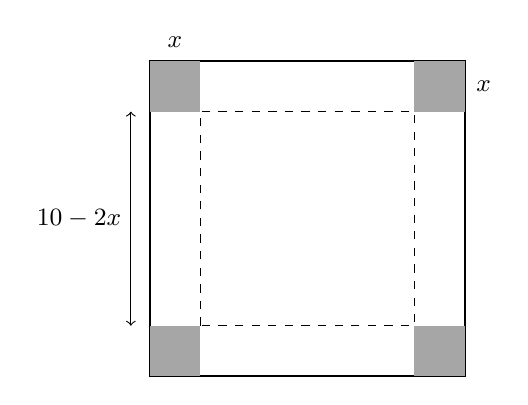
\begin{tikzpicture}[scale=0.4]
  \draw[thick] (0,0) rectangle (10,10);
  \foreach \p in {(0,0),(8.4,0),(0,8.4),(8.4,8.4)} \fill[gray!70] \p rectangle ++(1.6,1.6);
  \draw[dashed] (1.6,1.6) rectangle (8.4,8.4);
  \node at (0.8,10.6) {\small $x$}; \node at (10.6,9.2) {\small $x$};
  \draw[<->] (-0.6,1.6) -- (-0.6,8.4) node[midway,left] {\small $10 - 2x$};
\end{tikzpicture}
\end{center}
\ans
រកប្រវែងជ្រុង $x$ និងមាឌធំបំផុតនៃប្រអប់ ។ លក្ខខណ្ឌ $x > 0$ និង $10 - 2x > 0$ នោះ $0 < x < 5$ ។ មាឌនៃប្រអប់ $=$ ក្រឡាផ្ទៃបាត $\times$ កម្ពស់ ៖
\[
\begin{gathered}
f(x) = (10 - 2x)^2\times x = 4x^3 - 40x^2 + 100x,\\
0 < x < 5
\end{gathered}
\]
$f'(x) = 12x^2 - 80x + 100$ ។ $f'(x) = 0$ លុះត្រាតែ $12x^2 - 80x + 100 = 0$ ឬ $3x^2 - 20x + 25 = 0$ ។ $\Delta = 20^2 - 4(3)(25) = 100 = 10^2$ នោះ $x_1 = \dfrac{20 - 10}{6} = \dfrac{5}{3}$ ឬ $x_2 = \dfrac{20 + 10}{6} = 5$ ។
\begin{center}
\begin{tikzpicture}
  \tkzTabInit[lgt=1.6,espcl=2.4]{$x$ /0.8, $f'(x)$ /0.8, $f(x)$ /1.6}{$0$, $\frac{5}{3}$, $5$}
  \tkzTabLine{, +, z, -, z}
  \tkzTabVar{-/$0$, +/$\frac{2000}{27}$, -/$0$}
\end{tikzpicture}
\end{center}
$f$ មានអតិបរមាត្រង់ $x = \dfrac{5}{3}$ ហើយ $f\left(\dfrac{5}{3}\right) = \left(10 - 2\times\dfrac{5}{3}\right)^2\times\dfrac{5}{3} = \dfrac{2000}{27}$ ។

ដូច្នេះ ប្រអប់មានមាឌធំបំផុត កាលណាគេយក $x = \dfrac{5}{3}$ cm និងប្រអប់មានមាឌធំបំផុតគឺ $\dfrac{2000}{27}$ cm$^3$ ។

\begin{pro}
ស៊ីឡាំងមួយចារឹកក្នុងស្វ៊ែកាំ $R$ ។ \quad ក. រកកម្ពស់នៃស៊ីឡាំងដើម្បីឱ្យស៊ីឡាំងមានមាឌធំបំផុត ។ \quad ខ. រកមាឌធំបំផុតនៃស៊ីឡាំង ។
\ans
ក. កម្ពស់នៃស៊ីឡាំង $\dfrac{2\sqrt{3}}{3}R$ \quad ខ. $\dfrac{4\sqrt{3}}{9}\pi R^3$ ។
\end{pro}

\section{ចំណុចរបត់នៃខ្សែកោង}

\begin{example}[ឧទាហរណ៍]
គេឱ្យអនុគមន៍ $f(x) = x^3 - 3x^2$ ។
\begin{itemize}
  \item ដេរីវេទី $1$ ៖ $f'(x) = 3x^2 - 6x$ ។ បើ $f'(x) = 0$ នោះ $3x(x - 2) = 0$ ហើយ $x = 0$ ឬ $x = 2$ ។ ចំពោះ $x = 0 \Rightarrow f(0) = 0$ និងចំពោះ $x = 2 \Rightarrow f(2) = -4$ ។
  \item ដេរីវេទី $2$ ៖ $f''(x) = 6x - 6$ ។ បើ $f''(x) = 0 \Leftrightarrow 6x - 6 = 0 \Rightarrow x = 1$, $y = 1^3 - 3(1)^2 = -2$ ។
\end{itemize}
\end{example}
តារាងសញ្ញា $f''(x)$ និងតារាងអថេរភាព ៖
\begin{center}
\begin{tikzpicture}
  \tkzTabInit[lgt=1.6,espcl=2]{$x$ /0.8, $f''(x)$ /0.8}{$-\infty$, $1$, $+\infty$}
  \tkzTabLine{, -, z, +, }
\end{tikzpicture}

\begin{tikzpicture}
  \tkzTabInit[lgt=1.6,espcl=2]{$x$ /0.8, $f'(x)$ /0.8, $f(x)$ /1.6}{$-\infty$, $0$, $2$, $+\infty$}
  \tkzTabLine{, +, z, -, z, +, }
  \tkzTabVar{-/ , +/$0$, -/$-4$, +/ }
\end{tikzpicture}
\end{center}

\begin{center}
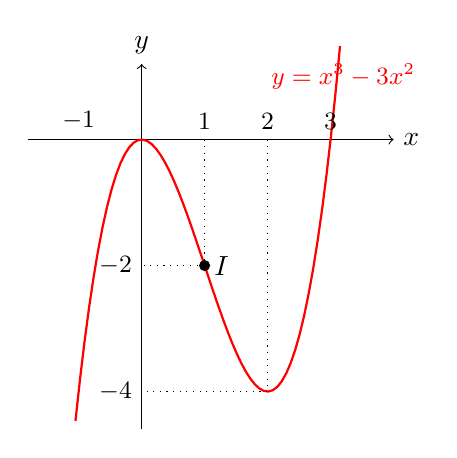
\begin{tikzpicture}[scale=0.8]
  \draw[->] (-1.8,0) -- (4,0) node[right] {$x$};
  \draw[->] (0,-4.6) -- (0,1.2) node[above] {$y$};
  \draw[thick,red,domain=-1.05:3.15,samples=60] plot (\x,{(\x)^3-3*(\x)^2});
  \fill (1,-2) circle (2.5pt) node[right] {$I$};
  \draw[dotted] (1,0) -- (1,-2) -- (0,-2) node[left] {\small $-2$};
  \draw[dotted] (2,0) -- (2,-4) -- (0,-4) node[left] {\small $-4$};
  \foreach \x in {-1,1,2,3} \node[above] at (\x,0) {\small $\x$};
  \node[red] at (3.2,1) {\small $y = x^3 - 3x^2$};
\end{tikzpicture}
\end{center}

តាមក្រាប គេសង្កេតឃើញថាខ្សែកោងប្ដូរពីប៉ោងទៅផតត្រង់ចំណុច $I(1, -2)$ ដែលហៅថាចំណុចរបត់នៃខ្សែកោងតាងអនុគមន៍ $f$ ។

\begin{formulaBox}[ជាទូទៅ]
ចំណុច $I(x_0, y_0)$ ជាចំណុចរបត់នៃខ្សែកោងតាងអនុគមន៍ កាលណាខ្សែកោងប៉ោងឬផតនៅលើ $[a, x_0]$ ហើយផតឬប៉ោងលើ $[x_0, b]$ ។ របៀបរកចំណុចរបត់នៃខ្សែកោងតាងអនុគមន៍ $f$ ៖
\begin{itemize}
  \item ជំហានទី $1$ ៖ រក $f''(x)$ ។
  \item ជំហានទី $2$ ៖ ដោះស្រាយសមីការ $f''(x) = 0$ ។
  \item ជំហានទី $3$ ៖ សិក្សាសញ្ញានៃ $f''(x)$ ។ បើ $f''(x)$ ដូរសញ្ញានៅសងខាង $x_0$ នោះខ្សែកោងមានចំណុចរបត់ $I(x_0, f(x_0))$ ។ បើ $f''(x)$ មិនដូរសញ្ញា នោះខ្សែកោងគ្មានចំណុចរបត់ទេ ។
\end{itemize}
\end{formulaBox}

\begin{note}[សម្គាល់]
ចំណុច $I(x_0, y_0)$ ជាចំណុចរបត់ លុះត្រាតែ $f(x_0) = y_0$ និង $f''(x_0) = 0$ (ហើយ $f''$ ដូរសញ្ញានៅសងខាង $x_0$) ។
\end{note}

\begin{example}[លំហាត់គំរូ]
រកចំណុចរបត់នៃខ្សែកោងតាង $y = x^3 - 3x + 1$ ។
\end{example}
\ans
ជំហានទី $1$ ៖ $y' = 3x^2 - 3$, $y'' = 6x$ ។ ជំហានទី $2$ ៖ $y'' = 6x = 0$ នោះ $x = 0$ ។ ជំហានទី $3$ ៖ សិក្សាសញ្ញានៃ $y'' = 6x$ ៖
\begin{center}
\begin{tikzpicture}
  \tkzTabInit[lgt=1.6,espcl=2]{$x$ /0.8, $y''$ /0.8}{$-\infty$, $0$, $+\infty$}
  \tkzTabLine{, -, z, +, }
\end{tikzpicture}
\end{center}
$y''$ ប្ដូរសញ្ញានៅសងខាង $x = 0$ ។ ចំពោះ $x = 0$, $y = y(0) = 1$ ។ ដូច្នេះ ចំណុច $I(0, 1)$ ជាចំណុចរបត់នៃខ្សែកោងតាងអនុគមន៍ ។

\begin{pro}
\begin{enumerate}[a]
  \item រកចំណុចរបត់នៃខ្សែកោងតាង $y = x^4 - 6x^2$ ។
  \item តើក្រាបតាង $y = \dfrac{1}{4}x^4 - \dfrac{1}{3}x^3 + \dfrac{1}{2}x^2 - 1$ មានចំណុចរបត់ឬទេ?
\end{enumerate}
\ans
ក. $y'' = 12x^2 - 12 = 0$ នាំឱ្យ $x = \pm 1$ ។ ចំណុចរបត់គឺ $(-1, -5)$ និង $(1, -5)$ \quad ខ. $y'' = 3x^2 - 2x + 1 > 0$ ជានិច្ច ដូច្នេះគ្មានចំណុចរបត់ទេ ។
\end{pro}

\section{ល្បឿននៃចលនាត្រង់}

ចំណុចមួយផ្លាស់ទីនៅលើបន្ទាត់ $L$ មួយ ។ បើគេយក $x$ ជាចម្ងាយចរនៃ $M$ បន្ទាប់ពី $t$ វិនាទី ក្រោយមកនោះ គេបាន $x$ ជាអនុគមន៍នៃ $t$ ហើយតាងដោយ $x = f(t)$ ។

\begin{center}
\begin{tikzpicture}[scale=0.9]
  \draw[->] (0,1) -- (8,1) node[right] {\small ចម្ងាយចរ};
  \draw[->] (0,0) -- (8,0) node[right] {\small ពេល};
  \node[left] at (0,1) {$L$}; \node[below] at (0,1) {\small $0$}; \node[below] at (0,0) {\small $0$};
  \fill (2.5,1) circle (2pt) node[above] {$M$};
  \node[below] at (2.5,1) {\small $x = f(t)$}; \node[below] at (5.5,1) {\small $f(t + \Delta t)$};
  \draw[dotted] (2.5,1) -- (2.5,-0.2) node[below] {$t$};
  \draw[dotted] (5.5,1) -- (5.5,-0.2) node[below] {$t + \Delta t$};
  \draw[<->] (2.5,0.25) -- (5.5,0.25) node[midway,above] {\small $\Delta t$};
\end{tikzpicture}
\end{center}

ល្បឿនមធ្យមនៃ $M$ ពីខណៈ $t$ ទៅ $t + \Delta t$ កំណត់ដោយ $\dfrac{\Delta x}{\Delta t} = \dfrac{f(t + \Delta t) - f(t)}{\Delta t}$ ។ បើ $\Delta t \to 0$ នោះគេតាង
\[ V = \lim_{\Delta t \to 0}\frac{\Delta x}{\Delta t} = \lim_{\Delta t \to 0}\frac{f(t + \Delta t) - f(t)}{\Delta t} \]
គេបាន $V = \dfrac{dx}{dt} = f'(t)$ ហៅថាល្បឿននៃ $M$ នៅខណៈ $t$ ។

\begin{example}[លំហាត់គំរូ]
ចំណុច $M$ មួយផ្លាស់ទីនៅលើបន្ទាត់ចំនួនចេញពីគល់អ័ក្ស ។ ចំណុច $M$ មានចម្ងាយចរ $x = t^3 - 6t^2 + 9t + 10$ នៅខណៈ $t$ វិនាទីក្រោយមក ។
\begin{enumerate}[a]
  \item រកល្បឿននៃចំណុច $M$ នៅខណៈ $\dfrac{1}{2}$ វិនាទីនិងនៅខណៈ $2$ វិនាទីក្រោយមក ។
  \item តើនៅខណៈណាដែលចំណុច $M$ ប្ដូរទិសដៅលើកដំបូងគេ ។
\end{enumerate}
\end{example}
\ans
\begin{enumerate}[a]
  \item តាង $V$ ជាល្បឿននៃ $M$ បន្ទាប់ពី $t$ វិនាទីក្រោយមក គេបាន $V = \dfrac{dx}{dt} = (t^3 - 6t^2 + 9t + 10)' = 3t^2 - 12t + 9$ ។

  នៅខណៈ $t = \dfrac{1}{2}\,s$ គេបាន $V\left(\dfrac{1}{2}\right) = 3\left(\dfrac{1}{2}\right)^2 - 12\left(\dfrac{1}{2}\right) + 9 = \dfrac{15}{4}$ ។ នៅខណៈ $t = 2\,s$ គេបាន $V(2) = 3\times 2^2 - 12\times 2 + 9 = -3$ ។
  \item ចំណុច $M$ ប្ដូរទិសដៅ កាលណាល្បឿន $V$ ប្ដូរសញ្ញា ។ បើ $V = 3t^2 - 12t + 9 = 0$ នោះ $t = 1$ ឬ $t = 3$ ។
  \begin{center}
  \begin{tikzpicture}
    \tkzTabInit[lgt=1.6,espcl=2]{$t$ /0.8, $V$ /0.8}{$0$, $1$, $3$, $+\infty$}
    \tkzTabLine{, +, z, -, z, +, }
  \end{tikzpicture}
  \end{center}
  តាមតារាងសញ្ញាល្បឿន $V$ ប្ដូរសញ្ញាលើកទី $1$ ត្រង់ខណៈ $t = 1\,s$ ។ ដូច្នេះ ចំណុច $M$ ប្ដូរទិសដៅលើកដំបូងគេត្រង់ខណៈ $t = 1\,s$ ។
\end{enumerate}

\begin{pro}
គេបោះបាល់មួយពីផ្ទៃដីឡើងទៅលើតាមទិសឈរដោយមានល្បឿនដើម $v_0 = 19.6\,m/s$ ។ ក្នុងរយៈពេល $t$ វិនាទីក្រោយមក បាល់ស្ថិតនៅកម្ពស់ $S = -4.9t^2 + 19.6t$ ពីផ្ទៃដី ។
\begin{enumerate}[a]
  \item រកល្បឿននៃបាល់ បន្ទាប់ពី $1$ វិនាទីក្រោយពីការបោះ ។
  \item រករយៈពេលដែលបាល់ស្ថិតនៅកម្ពស់ខ្ពស់បំផុត ហើយរកកម្ពស់នោះ ។
  \item រករយៈពេលដែលបាល់ស្ថិតនៅក្នុងលំហអាកាស ។
  \item រកចម្ងាយចរសរុបដែលបាល់បានផ្លាស់ទី ។
\end{enumerate}
\ans
ក. $v(1) = 9.8\,m/s$ \quad ខ. $t = 2\,s$, $S = 19.6\,m$ \quad គ. $0 < t < 4\,s$ \quad ឃ. $39.2\,m$ ។
\end{pro}

\section*{លំហាត់អនុវត្តន៍}
\begin{enumerate}[1]
  \item រកតម្លៃ $f'(-3)$, $f'(0)$ និង $f'(2)$ ដោយប្រើក្រាបតាងអនុគមន៍ $f$ ។ (បន្ទាត់ប៉ះត្រង់ $x = -3$ កាត់តាមចំណុច $(-5, 0)$ និងបន្ទាត់ប៉ះត្រង់ $x = 2$ កាត់តាមចំណុច $(4, 0)$ ។)

  \begin{center}
  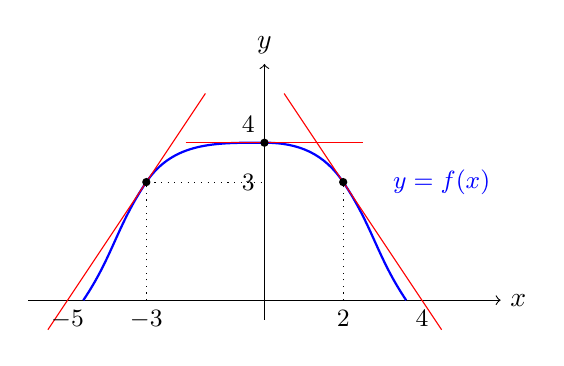
\begin{tikzpicture}[scale=0.5]
    \draw[->] (-6,0) -- (6,0) node[right] {$x$};
    \draw[->] (0,-0.5) -- (0,6) node[above] {$y$};
    \draw[thick,blue] (-4.6,0) to[out=56,in=236] (-3,3) to[out=56,in=180] (0,4) to[out=0,in=124] (2,3) to[out=-56,in=124] (3.6,0);
    \draw[red] (-5.5,-0.75) -- (-1.5,5.25);
    \draw[red] (0.5,5.25) -- (4.5,-0.75);
    \draw[red] (-2,4) -- (2.5,4);
    \fill (-3,3) circle (3pt); \fill (2,3) circle (3pt); \fill (0,4) circle (3pt);
    \draw[dotted] (-3,0) -- (-3,3) -- (0,3); \draw[dotted] (2,0) -- (2,3);
    \foreach \x in {-5,-3,2,4} \node[below] at (\x,0) {\small $\x$};
    \node[left] at (0,3) {\small $3$}; \node[above left] at (0,4) {\small $4$};
    \node[blue] at (4.5,3) {\small $y = f(x)$};
  \end{tikzpicture}
  \end{center}
  \ans
  $f'(-3) = \dfrac{3 - 0}{-3 - (-5)} = \dfrac{3}{2}$, \ $f'(0) = 0$ (បន្ទាត់ប៉ះដេក), \ $f'(2) = \dfrac{0 - 3}{4 - 2} = -\dfrac{3}{2}$ ។
  \item អនុគមន៍ $f(x) = 2x^3 - 16x + 11$ មានក្រាប $C$ ។
  \begin{enumerate}[a]
    \item រកសមីការបន្ទាត់ $L$ ដែលប៉ះក្រាប $C$ ត្រង់ចំណុច $A(2, -5)$ ។
    \item រកសមីការបន្ទាត់ដែលមានមេគុណប្រាប់ទិសស្មើ $-10$ ហើយប៉ះនឹងក្រាប $C$ ។
  \end{enumerate}
  \ans
  ក. $L : y = 8x - 21$ \quad ខ. $y = -10x + 7$ (ប៉ះត្រង់ $(1, -3)$) និង $y = -10x + 15$ (ប៉ះត្រង់ $(-1, 25)$) ។
  \item អនុគមន៍ $f(x) = 4x^3 + 9x^2 - 30x + 1$ មានក្រាប $C$ ។
  \begin{enumerate}[a]
    \item រកកូអរដោនេនៃគ្រប់ចំណុចប៉ះនៃក្រាប $C$ ដែលមានបន្ទាត់ប៉ះជាបន្ទាត់ដេក ។
    \item រកសមីការនៃបន្ទាត់ប៉ះទាំងនោះ ។
  \end{enumerate}
  \ans
  ក. $f'(x) = 6(2x + 5)(x - 1) = 0$ ៖ ចំណុចប៉ះ $(1, -16)$ និង $\left(-\dfrac{5}{2}, \dfrac{279}{4}\right)$ \quad ខ. $y = -16$ និង $y = \dfrac{279}{4}$ ។
  \item អនុគមន៍ $y = 3x^2 - 4x + 1$ កំណត់នៅលើ $\mathbb{R}$ និងមានក្រាប $C$ ។
  \begin{enumerate}[a]
    \item រកសមីការបន្ទាត់ប៉ះនឹង $C$ ហើយកែងនឹងបន្ទាត់ $y = -\dfrac{x}{5} + 2$ ។
    \item រកសមីការបន្ទាត់ប៉ះនឹង $C$ ហើយស្របនឹងបន្ទាត់ $y = x + 5$ ។
  \end{enumerate}
  \ans
  ក. $y = 5x - \dfrac{23}{4}$ \quad ខ. $y = x - \dfrac{13}{12}$ ។
  \item អនុគមន៍ $f(x) = x^3 - 3x$ កំណត់នៅលើ $\mathbb{R}$ និងមានក្រាប $C$ ។
  \begin{enumerate}[a]
    \item រកសមីការបន្ទាត់ប៉ះនឹងក្រាប $C$ ត្រង់ចំណុច $A$ ដែលមានអាប់ស៊ីស $a$ ។
    \item បន្ទាត់ប៉ះត្រង់ $A$ កាត់ក្រាប $C$ ម្ដងទៀតត្រង់ $B$ ។ រកអាប់ស៊ីសនៃ $B$ ។
  \end{enumerate}
  \ans
  ក. $y = (3a^2 - 3)x - 2a^3$ \quad ខ. $x^3 - 3x - (3a^2 - 3)x + 2a^3 = (x - a)^2(x + 2a) = 0$ ដូច្នេះអាប់ស៊ីសនៃ $B$ គឺ $-2a$ $(a \ne 0)$ ។
  \item សិក្សាទិសដៅអថេរភាព រកអតិបរមា និងអប្បបរមា ហើយសង់តារាងអថេរភាពនៃអនុគមន៍នីមួយៗដូចខាងក្រោម ៖
  \begin{tasks}(3)
    \task $y = -x^3 + 3x^2 + 4$
    \task $y = x(x - 3)^2$
    \task $y = -x^2(x - 1)^2$
  \end{tasks}
  \ans
  ក. ចុះលើ $(-\infty, 0)$ និង $(2, +\infty)$, កើនលើ $(0, 2)$ ៖ អប្បបរមាធៀប $y(0) = 4$, អតិបរមាធៀប $y(2) = 8$ ។

  ខ. $y' = 3(x - 1)(x - 3)$ ៖ កើនលើ $(-\infty, 1)$ និង $(3, +\infty)$, ចុះលើ $(1, 3)$ ៖ អតិបរមាធៀប $y(1) = 4$, អប្បបរមាធៀប $y(3) = 0$ ។

  គ. $y' = -2x(x - 1)(2x - 1)$ ៖ កើនលើ $(-\infty, 0)$ និង $\left(\dfrac{1}{2}, 1\right)$, ចុះលើ $\left(0, \dfrac{1}{2}\right)$ និង $(1, +\infty)$ ៖ អតិបរមាធៀប $y(0) = y(1) = 0$, អប្បបរមាធៀប $y\left(\dfrac{1}{2}\right) = -\dfrac{1}{16}$ ។
  \item អនុគមន៍ $f(x) = x^3 + 3ax^2 + 3bx + 2$ មានអតិបរមាធៀបត្រង់ $x = 1$ និងមានអប្បបរមាធៀបត្រង់ $x = 2$ ។
  \begin{enumerate}[a]
    \item រកតម្លៃនៃចំនួនពិត $a$ និង $b$ ។
    \item រកផលដករវាងតម្លៃអតិបរមាធៀបនិងអប្បបរមាធៀបនៃ $f$ ។
  \end{enumerate}
  \ans
  ក. $a = -\dfrac{3}{2}$, $b = 2$ \quad ខ. $f(1) - f(2) = \dfrac{9}{2} - 4 = \dfrac{1}{2}$ ។
  \item អនុគមន៍ $f(x) = x^4 + 29$ និង $g(x) = 4x^3$ មានក្រាប $C_1$ និង $C_2$ ។ បន្ទាត់ $D$ ស្របអ័ក្សអរដោនេ កាត់ក្រាប $C_1$ និង $C_2$ រៀងគ្នាត្រង់ $A$ និង $B$ ។ រកប្រវែងអប្បបរមានៃអង្កត់ $[AB]$ ។
  \ans
  $AB = x^4 - 4x^3 + 29$ មានអប្បបរមាត្រង់ $x = 3$ ។ ប្រវែងអប្បបរមា $AB = 2$ ។
  \item បន្ទះស័ង្កសីរាងត្រីកោណសម័ង្សមួយមានជ្រុងប្រវែង $a$ ។ គេកាត់យកចេញពីផ្នែកត្រង់កំពូលទាំងបីនូវចតុកោណប៉ុនៗគ្នា (ជ្រុងប្រវែង $x$ តាមជ្រុងត្រីកោណ និងមានមុំកែងពីរ) ។ គេបត់ផ្នែកនៅសល់ឱ្យបានជាប្រអប់មួយដែលមានរាងជាព្រីសត្រីមុខនិយ័ត ហើយគ្មានគម្រប ។ រកតម្លៃ $x$ ដើម្បីឱ្យប្រអប់មានមាឌធំបំផុត ។

  \begin{center}
  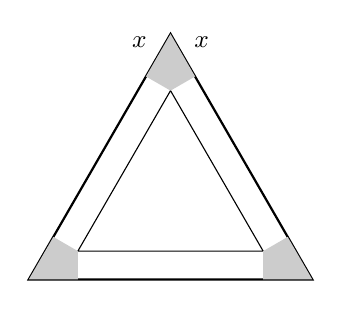
\begin{tikzpicture}[scale=0.6]
    \coordinate (A) at (0,0); \coordinate (B) at (6,0); \coordinate (C) at (3,5.196);
    \draw[thick] (A) -- (B) -- (C) -- cycle;
    \coordinate (a1) at (1.039,0.6); \coordinate (b1) at (4.961,0.6); \coordinate (c1) at (3,3.996);
    \draw (a1) -- (b1) -- (c1) -- cycle;
    \fill[gray!40] (A) -- (1.039,0) -- (a1) -- (0.52,0.9) -- cycle;
    \fill[gray!40] (B) -- (4.961,0) -- (b1) -- (5.48,0.9) -- cycle;
    \fill[gray!40] (C) -- (2.48,4.296) -- (c1) -- (3.52,4.296) -- cycle;
    \node[above left] at (2.7,4.7) {\small $x$}; \node[above right] at (3.3,4.7) {\small $x$};
  \end{tikzpicture}
  \end{center}
  \ans
  កម្ពស់ប្រអប់ $h = \dfrac{x}{\sqrt{3}}$ និងជ្រុងបាត $a - 2x$ ។ មាឌ $V = \dfrac{\sqrt{3}}{4}(a - 2x)^2\cdot\dfrac{x}{\sqrt{3}} = \dfrac{1}{4}x(a - 2x)^2$, $0 < x < \dfrac{a}{2}$ ។ $V' = \dfrac{1}{4}(a - 2x)(a - 6x) = 0$ នាំឱ្យ $x = \dfrac{a}{6}$ ។ មាឌធំបំផុត $V = \dfrac{a^3}{54}$ ។
  \item ថ្មមួយដុំបានធ្លាក់ពីកម្ពស់ $88.2$ ម៉ែត្រតាមទិសឈរសំដៅមកផ្ទៃដី ។ ក្នុងរយៈពេល $t$ វិនាទីក្រោយមក ដុំថ្មនោះធ្លាក់បានចម្ងាយ $9.8t^2$ ម៉ែត្រ ។
  \begin{enumerate}[a]
    \item តើក្នុងរយៈពេលប៉ុន្មានវិនាទីក្រោយមកទើបដុំថ្មធ្លាក់ប៉ះផ្ទៃដី ។
    \item រកល្បឿនធ្លាក់នៃដុំថ្មនៅខណៈ $2$ វិនាទីដំបូង ។
    \item រកល្បឿនធ្លាក់នៃដុំថ្មនៅពេលធ្លាក់ប៉ះផ្ទៃដី ។
  \end{enumerate}
  \ans
  ក. $9.8t^2 = 88.2$ នាំឱ្យ $t = 3$ វិនាទី \quad ខ. $v = 19.6t$, $v(2) = 39.2\,m/s$ \quad គ. $v(3) = 58.8\,m/s$ ។
  \item គេបាញ់វត្ថុមួយតាមទិសឈរពីផ្ទៃដីសំដៅទៅលើអាកាស ដោយមានល្បឿនដើម $V_0 = 39.2\,m\cdot s^{-1}$ ហើយមានចម្ងាយចរ $S = -4.9t^2 + 39.2t$ គិតជាម៉ែត្រពីផ្ទៃដីបន្ទាប់ពី $t$ វិនាទីក្រោយមក ។
  \begin{enumerate}[a]
    \item រកល្បឿននៃវត្ថុនៅខណៈ $t$ បន្ទាប់ពីការបាញ់
    \item តើនៅពេលណាដែលវត្ថុស្ថិតនៅកម្ពស់ខ្ពស់បំផុត ។ រកកម្ពស់នោះ ។
    \item រករយៈពេលដែលវត្ថុស្ថិតក្នុងលំហអាកាស ។
    \item រកចម្ងាយចរសរុបនៃវត្ថុ ។
  \end{enumerate}
  \ans
  ក. $V = -9.8t + 39.2$ \quad ខ. $t = 4\,s$, កម្ពស់ $78.4\,m$ \quad គ. $0 < t < 8\,s$ \quad ឃ. $156.8\,m$ ។
\end{enumerate}
